%!TEX root = proposal.tex
%\addbibresource{bibliography.bib}
%-----------------------------------------------------------------------------
\section{Proposed Work}\label{sect:proposedWork}
%-----------------------------------------------------------------------------


%----------------------------------------------------------------------------
\subsection{Approach}
%----------------------------------------------------------------------------

The use of a high-level language like Galois with dynamic work generation and dynamic dependencies means that 
static scheduling approaches found in traditional high-level synthesis no longer apply. The Galois programming model semantics coupled with the 
Galois concurrent library components means that the user does not deal with issues such as atomicity, 
scheduling, work balancing, worklist spilling, prefetching, and more. In addition, the Galois HLS compiler is responsible for the 
generation of custom pipelines. These pipelines are multithreaded, in which each pipeline stage is working 
on a different thread. Unlike pipelines generated by traditional HLS tools such as Vivado, instructions flowing 
through the pipeline are issued dynamically as work items arrive. Pipeline stages may stall based on the control 
flow and variable latency accelerators. The compiler is responsible for generating the proper stall and forwarding 
logic to preserve correctness.

Due to pointer-chasing memory patterns and large memory footprint of graph applications, traditional memory 
hierarchies found in general purpose processors tend to perform poorly. This is where FPGAs can be much more effective. 
By tailoring the Galois microarchitecture to be able to saturate the available memory bandwidth of the system, an FPGA 
platform can outperform a general purpose CPU platform with similar bandwidth since the CPU often cannot effecitvely 
exploit all the available bandwidth in the system.

While the Galois for FPGA framework requires a substantial amount of work implementing transactional memory semantics, 
this is outside the scope of my thesis. My labmate Xiaoyu Ma will be implementing this as part of his thesis.


\subsection{Proposed User Workflow}

Using Galois for FPGA is similar to using Galois for software. The user writes a Galois program using the Galois library modes 
and the \textbf{foreach} Galois construct. This Galois program will have different syntax to the current Galois SW 
implementation in C++, but that's because the authors of Galois did not wish to implement a compiler, instead 
implementing Galois as several libraries within C++. In addition, instead of using C++, the Galois HLS compiler will use C 
and have the same restrictions as a standard HLS tool such as the lack of dynamic memory allocation outside of the 
Galois constructs, as I plan on implementing Galois by augmenting an existing HLS tool. Pragmas to provide high-level 
microarchitectural hints may be required, but will be avoided if possible.

After writing the Galois program, the user calls the Galois HLS compiler. The compiler generates the custom 
multithreaded pipelined engine code executing the \textbf{foreach} block and connects the engines to the Galois 
microarchitecture implemented in Bluespec. Parameters are passed to the Galois microarchitecture by the compiler with 
possible user input. Either the user or the compiler will tweak the parameters until the design meets timing and 
routing FPGA constraints.

\subsection{Galois Microarchitecture}

\begin{figure}
\centering
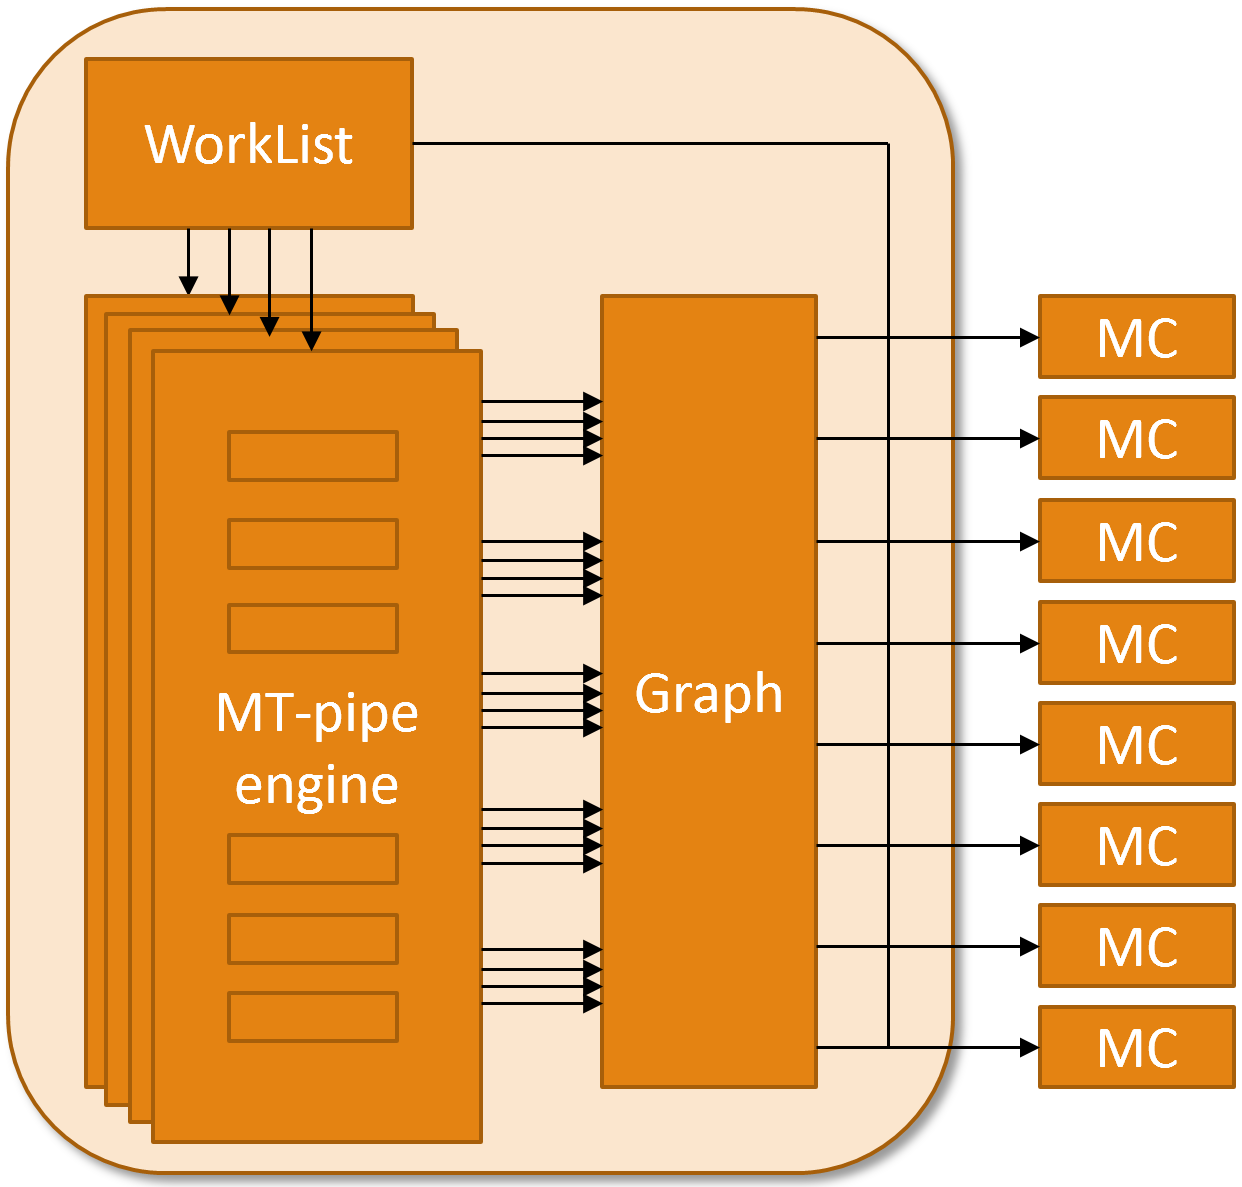
\includegraphics[width=6.5cm, keepaspectratio]{pics/uarch.png}
\caption{The Galois microarchitecture}
\label{fig:uarch}
\end{figure}

The Galois microarchitecture is a high-throughput packet processor that interfaces with custom engine code generated 
by the Galois HLS compiler as seen in Figure \ref{fig:uarch}. It consists of four major components: the custom engine code, the 
instantiated worklist, the instantiated graph module, and the surrounding infrastructure logic. The worklist and graph 
module variant and parameters are chosen by the user through explicit instantiation in the user code. Some other 
parameters may be set by the Galois HLS compiler based on the number of engines generated and the Galois library calls 
made by the engines. The surrounding infrastructure logic provides glue logic for the components and is custom to the 
target FPGA platform.

The Galois microarchitecture bears many similarities to Tera \cite{tera}. Like Tera, the Galois microarchitecture is 
a heavily multithreaded throughput system without data caches. However, there are several key differences. Since the 
Galois engines are custom-generated for the target program, they can achieve a high throughput per engine at low power. 
Depending on the application and available bandwidth in the FPGA platform, instead of 
needing 256 cores like Tera, the Galois microarchitecture only needs tens of engines or even fewer to fully saturate 
memory bandwidth. In addition, Galois supports a dedicated hardware priority scheduler and transactional memory 
framework.

\subsubsection{Worklist}

\begin{table}
\begin{tabular}{ | l | l | }
  \hline
  \textbf{Method} & \textbf{Description} \\
  \hline
  void enq(WorkItem work) & Enqueue work item into worklist \\
  \hline
  void enq(Priority p, WorkItem work) & Enqueue work item into worklist with priority p\\
  \hline
  WorkItem deq() & Dequeue and return work item from worklist \\
  \hline
\end{tabular}
\caption{Worklist interface}
\label{table:worklist}
\end{table}

The worklist library component performs work scheduling within the Galois microarchitecture. In the Galois programming 
model, the user writes a Galois kernel consisting of a foreach loop, wherein each loop iteration dequeues a work item 
from the worklist and may enqueue any number of additional work items to the worklist. The worklist therefore presents 
a simple FIFO interface is exposed to the programmer shown in Table \ref{table:worklist}, but behind the curtains it 
must perform dynamic work scheduling across tens to hundreds of threads on multiple engines across multiple FPGAs. In 
addition, the size of the worklist is unbounded, so the worklist must support dynamic fills and spills to memory. 
Proper care must be taken to ensure that work is balanced evenly using optimizations like work stealing, with 
optimizations such as streaming and double buffering to ensure memory spills and fills do not bottleneck the engines.

The standard worklist supports a simple FIFO schedule. However, many algorithms such as SSSP converge much faster 
given a priority schedule \cite{galoisOrdering}. Current state-of-the-art for software worklists require the user to 
specify a static priority algorithm, such as the bucket size for SSSP. Various priorities have been proposed for 
different algorithms, optimizing not only for convergence speed but also cache hit rate. Unfortunately, the best 
priority not only depends on the algorithm but also on the host architecture and shape of the input graph. In 
addition, I strongly suspect that the optimal priority may change as the amount of parallelism in the system 
dynamically grows and shrinks during execution.

\subsubsection{Worklist priority scheduling}

To further improve work efficiency, I propose the use of dynamic priority scheduling. Dynamic priority scheduling will 
utilize microarchitectural performance counters to optimize for convergence speed when possible. For example, in SSSP 
delta-stepping, the size of the bucket should be as small as possible while still providing enough work to avoid 
backpressuring the engines. By monitoring the amount of work in each bucket and the rate of engine work consumption, the 
worklist can dynamically adjust bucket size to provide near-optimal performance.

Other algorithms will require different types of scheduling to maximize the rate of convergence. Ideally, choosing the 
correct schedule should be determined by the microarchitecture. I will explore the possibility of determining the right 
scheduling algorithm to use and its parameters to maximize for performance, 
which is a function of the convergence rate and rate of work item completion.

\subsubsection{Graph}

\begin{table}
\begin{tabular}{ | l | l | }
  \hline
  \textbf{Method} & \textbf{Description} \\
  \hline
  void startTransaction() & Start atomic transaction \\
  \hline
  void endTransaction() & End atomic transaction \\
  \hline
  Node readNode(NodeID id) & Read node from graph \\
  \hline
  Edge readEdge(EdgeID id) & Read edge from graph \\
  \hline
  EdgeIterator readEdges(Node node) & Galois iterator for each edge in graph node\\
  \hline
  Bool cas(Payload\& cmpVal, Payload swapVal) & Compare-and-swap, returns success and old val\\
  \hline
  void writeNodePayload(Payload p) & Write node payload \\
  \hline
  void writeEdgePayload(Payload p) & Write edge payload \\
  \hline
\end{tabular}
\caption{Graph interface}
\label{table:graph}
\end{table}

Compiler-emitted Galois kernel engines do not interface directly with memory. Instead, they interface with the Graph 
concurrent library module, which handles preserving atomicity, interfacing with the underlying host memory fabric, and 
handling multiple memory operations in flight across multiple memory channels. The graph interface is shown in Table 
\ref{table:graph}. Note that the user will not have to explicitly call startTransaction() and endTransaction(). 
Instead, the Galois HLS compiler will emit these operations in place of the user. However, if the user wishes to 
perform low-level optimizations, he or she may choose to forgo the use of transactional memory and instead manually 
call the provided compare-and-swap atomic operation.

Note that this graph library module provided is a local computation graph, i.e. the graph structure does not change. 
The user is only able to modify the node payload contents, i.e. the local data associated with each node. This 
limitation still supports large number of graph algorithms, including SSSP, breadth-first search, preflow push, 
PageRank, and many more. I will investigate supporting mutable graphs using a simple hardware memory allocator and 
garbage collector.

\subsubsection{Galois Infrastructure}

The Galois infrastructure consists of glue logic, buffering, and flow control for the engines, worklist, and graph. 
Graph and worklist operations must be converted from generic memory operations to the interface required for running 
on that particular FPGA platform. Arbitration is required between the worklist and graph, as well as with the parallel 
workers within the worklist and graphs themselves. The infrastructure must balance requests between the available 
memory channels on the host and guarantee forward progress, as well as performance optimizations such as memory 
request balancing (either static or dynamic) across the memory channels. As each FPGA platform has its own unique 
memory interface, a new Galois infrastructure must be designed for every FPGA platform. The current infrastructure is 
designed to exploit the Convey MX-100 platform's atomic memory operations and multi-FPGA environment, 
which many platforms do not support.



\subsection{Galois HLS compiler}

For my thesis, I plan on augmenting an existing HLS compiler to support the \textbf{foreach} Galois construct as well 
as the Galois concurrent worklist and graph library modules. A good candidate is LegUp \cite{legupMT}, an HLS compiler 
built on top of LLVM. The Galois HLS compiler should detect the \textbf{foreach} construct and call specialized code 
routines to perform the appropriate pipelining. As there are loops in Galois code, e.g. to iterate over a 
node's edges, the compiler must generate the appropriate code to handle the flow control and deadlock 
avoidance. The compiler will only generate the engine, i.e. the \textbf{foreach} loop body converted to hardware. After engine 
generation, the compiler instantiates and connects the Galois microarchitecture surrounding the engine from its set of 
Galois library components.

The focus of this proposal has been on the microarchitecture. I have hand-designed a fully pipelined engine to handle 
SSSP and integrates with the Galois infrastructure, including the worklist and graph library components. The goal is 
for the compiler to generate comparable code.